\chapter{はじめに}

\section{開発背景}

近年,PC,サーバ,組み込みシステム等,用途を問わずマルチプロセッシングシステムの利用が進んでいる.
その背景には,シングルプロセッサの高クロック化による性能向上効果の停滞や,それに伴う消費電力・発熱の増大がある.
マルチプロセッシングシステムでは処理の並列性を高めることにより性能向上を実現するため,消費電力の増加を抑えることが出来る.
組み込みシステムにおいては,機械制御とGUIなど要件の異なるサブシステム毎にプロセッサを使用する例があるなど,従来から複数のプロセッサを用いるマルチプロセッサシステムが存在していたが,部品点数の増加によるコスト増を招くため避ける方向にあった.
しかしながら,近年は,1つのプロセッサ上に複数の実行コアを搭載したマルチコアプロセッサの登場により低コストで利用することが可能になり,低消費電力要件の強い組み込みシステムでの利用が増加している.

マルチコアプロセッサ環境でソフトウェアを開発する際に問題になる点として,デバッグの困難さが挙げられる.
これは,マルチコアプロセッサ環境では,従来のブレークポイントやステップ実行を用いたデバッグの挙動が,シングルプロセッサ環境における場合と異なるからである.
たとえば,複数のコアで実行される可能性のあるコードにブレークポイントを置きデバッグを行う場合,ブレーク後にステップ実行を行い処理を追う最中に,他のコアのブレークにより中断される可能性があるため,ブレーク後にブレークポイントを一時的に削除する必要があり,頻繁にブレークポイントの設置,削除を行わなければならなくなる.
また,マルチコアプロセッサ環境では,特殊な状況下でのみ起こるバグが発生する可能性がある.その場合,原因を特定するのは通常困難である.
なぜならば,マルチコアプロセッサ環境では,特別な制御を行わない限り各コアが非同期的に並列動作するため,バグの発生を再現することが難しいからである.
また,再現が可能であったとしても,原因を特定するためには,バグが発生するまでの過程をすべてのコアの実行状況を監視しながら行う必要があり,シングルプロセッサ環境の場合に比べ非常に煩雑になる.

一方,マルチコアプロセッサ環境で有効なデバッグ手法としてトレースログの解析によるデバッグがある.
これは,プログラムの実行中に,デバッグの判断材料となる情報をログとして出力することによりプログラムの動作を確認する手法である.
ログの出力元としては,OSやICE,シミュレータなどがあり,情報の粒度もアプリケーションレベル,タスクレベル,カーネルレベル,ハードウェアレベルなど様々である.

しかしながら,トレースログを開発者が直接扱うのは困難である場合が多い.
これは,ログの情報の粒度が細かくなるほど単位時間あたりのログの量が増える傾向にあり,膨大なログから所望の情報を探し出すのが困難であることや,各コアのログが時系列に分散して記録されるため,逐次的にログを解析することが困難であるからである.
そのため,トレースログの解析を支援するツールが要求されており,ログを解析し統計情報として出力したり,可視化表示することで開発者の負担を下げる試みが行われている.

\section{既存のトレースログ可視化ツール}

既存のトレースログ可視化表示ツールとしては,ICE付属のデバッガソフトウェアや,組み込みシステム向け統合開発環境の一部,カーネルトレースツールのGUI,波形表示用ツールの流用などがある.

本節では,これら既存のトレースログ可視化ツールについて説明した後,これらの問題点について指摘する.

\subsection{JTAGエミュレータ付属デバッガソフトウェア}

JTAGエミュレータとは,オンチップ・エミュレータの一種であり,基板上にプロセッサを実装した状態でプログラムのデバッグを行うことのできる装置である.
主に組み込みシステムでのソフトウェア開発に使用され,ターゲットコンピュータとJTAGエミュレータをデバッグ用のインターフェイスで接続し,JTAGエミュレータとホストコンピュータをEthernetやシリアルポートで接続することで,ターゲットコンピュータ上でプログラムを実行しながらホストコンピュータでデバッグを行うことができる.
ホストコンピュータでは,JTAGエミュレータ付属のデバッガソフトウェアを使用してデバッグを行うが,そのソフトウェアにトレースログを可視化する機能が含まれている場合がある.
図\ref{fig:PARTNER-JET}に,京都マイクロコンピュータ株式会社のJTAGエミューレータPARTNER-Jet\cite{PARTNER-JET}に付属するデバッガソフトウェアの可視化機能であるイベントトラッカーのスクリーンショットを示す.

JTAGエミューレータ付属デバッガソフトウェアの一機能としての可視化ツールは,その性質からターゲットとなるOSやプロセッサが限定されてしまう.また,可視化表示したい情報も提供されているものに限られるなど,可視化ツールとしては汎用性,拡張性に乏しい.

\begin{figure}[p]
\begin{center}
\includegraphics[height=9cm]{img/PARTNER-JET.eps}
\caption{PARTNER-JET イベントトラッカー}
\label{fig:PARTNER-JET}
\end{center}
\end{figure}

\subsection{組み込みOS向けの統合開発環境}

QNX Software Systems社は,自社の組み込みリアルタイムオペレーティングシステムQNXの統合開発環境としてQNX Momenticsを販売している.QNX Momenticsにはシステムプロファイラとして,システムコールや割込み,スレッド状態やメッセージなどを可視化するQNX System Profiler\cite{QNXMomentics}という機能を提供している.図\ref{fig:QNXSystemProfiler}にQNX System Profilerのスクリーンショットを示す.

また,イーソル株式会社はT-Kenel/$\mu$ITRONベースシステムの統合開発環境としてeBinder\cite{eBinder}を販売している.eBinderにはイベントログ取得・解析ツールとしてEvenTrekが付属しており,システムコール,割込み,タスクスイッチ,タスク状態遷移などを可視化することが出来る.図\ref{fig:EvenTrek}にQNX System Profilerのスクリーンショットを示す.

このように,商用の組み込みOS向けの統合開発環境にはOSの実行履歴を可視化表示する機能が搭載されている場合がある.しかしながらこれらは,各ベンダーが自社OSの競争力を高めるために提供されているものであり,当然ながら可視化表示に対応するOSは自社提供のものに限られている.
また,可視化表示する情報も提供するものに限られており,表示のカスタマイズ機能もそれほど自由度は高くはない.

\begin{figure}[p]
\begin{center}
\includegraphics[height=9cm]{img/QNXSystemProfiler.eps}
\caption{QNXSystemProfiler}
\label{fig:QNXSystemProfiler}
\end{center}
\end{figure}

\begin{figure}[p]
\begin{center}
\includegraphics[height=9cm]{img/EvenTrek.eps}
\caption{eBinder EvenTrek}
\label{fig:EvenTrek}
\end{center}
\end{figure}

\subsection{カーネルトレースツールのGUI}

これまでに,パフォーマンスチューニングや障害解析を目的として,オペレーティングシステムの実行トレースを取得するソフトウェアがいくつか開発されている.
Linux用のトレースツールとしてはLKST\cite{LKST},SystemTap\cite{SystemTap},LTTng\cite{LTTng}などがあり,Solaris用にはDtrace\cite{Dtrace}がある.
これらトレースツールは,主にカーネル内にフックを仕込みカーネル内部状態をユーザー空間に通知する機能,通知をログとして記録する機能を提供している.また,ログを分析・提示するGUIソフトウェアとして専用の可視化ツールを提供している場合が多い.
たとえば,LTTngにはLTTV\cite{LTTV}が,DTraceにはChime\cite{Chime}が専用の可視化ツールとして提供されている.
図\ref{fig:LTTV}にLTTVのスクリーンショットを,図\ref{fig:Chime}にChimeのスクリーンショットを示す.

これら,カーネルトレースツールのGUIソフトウェアは,主に,カーネルの内部状態を統計情報として出力することにより,ボトルネックを探したり,障害の要因を探る目的で使用されるが,ソフトウェアのデバッグを目的に使用することもできる.
DTraceなどはログ出力のためのカーネルフックポイントを独自のスクリプト言語を用いて制御できるなど,任意の情報をソフトウェアの実行から取得することができる.
しかしながら,取得したログを任意の図形で可視化する手段は提供されておらず,テキスト形式での確認となる.
また,可視化表示する際のログの形式は,そのOSのトレースツールが出力する形式に依存するため,他のOSのトレースを可視化することはできない.

\begin{figure}[p]
\begin{center}
\includegraphics[height=9cm]{img/LTTV.eps}
\caption{LTTV}
\label{fig:LTTV}
\end{center}
\end{figure}

\begin{figure}[p]
\begin{center}
\includegraphics[height=9cm]{img/Chime.eps}
\caption{Chime}
\label{fig:Chime}
\end{center}
\end{figure}

\subsection{波形表示ツールの流用}

任意のOS,アプリケーションのトレースログを可視化表示する手段として,波形表示ツールを流用する方法がある.
波形表示ツールとは,Verilog等のデジタル回路設計用論理シミュレータの実行ログを波形で表示するソフトウェアのことを指す.
デジタル回路設計用論理シミュレータの実行ログには,VCD(Value Change Dump)形式というオープンなファイルフォーマットが提供されている.
そのため,任意のログをVCD形式として出力することにより,これらのツールで可視化表示することが可能になる.
図\ref{fig:GTKWave}に,VCD形式のログの可視化に対応した波形表示ツールGTKWaveのスクリーンショットを示す.

波形表示ツールを流用する方法では,任意のログをオープンフォーマットなファイル形式に変換することによりログの形式に依存せずに利用できる反面,表示能力に限界があり,複雑な可視化表現は難しい.

\begin{figure}[p]
\begin{center}
\includegraphics[height=9cm]{img/GTKWave.eps}
\caption{GTKWave}
\label{fig:GTKWave}
\end{center}
\end{figure}

\subsection{既存のトレースログ可視化ツールの問題点}

既存のトレースログ可視化ツールは,可視化ツールとして単体で存在しているわけではなく,トレースログを出力するソフトウェアの一部として提供されている.
そのため,読み込めるログの形式が出力ソフトウェアに依存し,ターゲットOS,ターゲットCPUが制限されてしまっている.
読み込むログの形式を制限しないためには,波形表示ツールのように可視化ツール用のオープンなログ形式を定める必要があると考えられるが,現状,公表されているものではそのようなものは確認できていない.
ログ形式の標準化としては,syslog\cite{RFC3164}と呼ばれる,ログメッセージをIPネットワーク上で転送するための標準規格がRFC3164として策定されており,その一部にログ形式について規定されている.しかしながら,syslogにおけるログ形式は,時刻の最小単位が秒であり,デバッグを目的に利用するには粒度が荒く,また,メッセージ内容がフリーフォーマットであるなど,自由度が高すぎるため,可視化ツールが読み込むログの標準形式としては不適切である.

既存のトレースログ可視化ツールのもうひとつの問題点としては,可視化表示の項目や形式が,提供されているものに限られていることが挙げられる.
これは,ログのターゲットや可視化の目的に合わせて可視化表現が最適化されているためである.
また,既存のトレースログ可視化ツールで可視化表示の項目を追加,変更したり,可視化表現をカスタマイズする機能を搭載するものは確認できていない.

\section{開発目的と内容}

前節で説明したとおり,既存のトレースログ可視化ツールには,オープンなログ形式がないことによりターゲットが限定されている点,可視化表示項目がターゲットにより固定されている点の2つの問題点があることを指摘した.
そこで我々は,これらの問題点を解決し,汎用性,拡張性を備えたトレースログ可視化ツールを開発することを目的とし,成果物として TraceLogVisualizer (TLV) を開発した.また,その過程でトレースログの標準形式を提案した.

問題解決のためにTLVが実装した機能は,トレースログの標準形式への変換と可視化表示項目のプラグイン化である.
トレースログを標準形式トレースログに変換することにより,あらゆるトレースログがTLVで可視化表示可能となる.

\section{論文の構成}
本節では本論文の構成を述べる.

2章では,TLVの設計について述べる.
ここでは,問題解決のために開発方針をどのように設定したかを述べ,具体的な解決策をどのように設計したかを述べる.
3章では,TLVの実装について述べる.
2章で述べた設計をメカニズムとしてどのように実現しているかを,プロセスとインターフェイスに分けて説明する.
4章では,TLVを利用した例を示し,その有効性について言及している.
5章ではTLVを開発するにあたり,どのような開発プロセスを用いたのかを述べている.
最後に6章で本論文のまとめと今後の展望と課題について述べる.